\documentclass{sig-alternate}
\graphicspath{{graphics/}}
\usepackage[hang]{subfigure}
%\usepackage{listings}
%\newcommand{\newlisting}[2]{\begin{lstlisting}[frame=trbl,caption={#1},label={#2},numbers=left,captionpos=b,float={ht}]{}}
\usepackage{mdwlist}
%\usepackage{savetrees}

\begin{document}
%\lstset{basicstyle=\tiny, numberstyle=\tiny}


% --- Author Metadata here ---
\conferenceinfo{WOODSTOCK}{'97 El Paso, Texas USA}
\CopyrightYear{2009} % Allows default copyright year (200X) to be over-ridden - IF NEED BE.
\crdata{0-12345-67-8/90/01}  % Allows default copyright data (0-89791-88-6/97/05) to be over-ridden - IF NEED BE.
% --- End of Author Metadata ---

\title{Adaption of XCS to predator/prey scenarios}
\subtitle{[Extended Abstract]}
\numberofauthors{3}
\author{
\alignauthor
Clemens Lode\\
    \email{clemens@lode.de}
\alignauthor
Urban Richter\\
    \affaddr{Karlsruhe Institute of Technology}\\
    \affaddr{Institute AIFB}\\
    \affaddr{76128 Karlsruhe, Germany}\\
    \email{urban.richter@kit.edu}\\
\alignauthor
Hartmut Schmeck\\
       \affaddr{Karlsruhe Institute of Technology}\\
       \affaddr{Institute AIFB}\\
       \affaddr{76128 Karlsruhe, Germany}\\
       \email{hartmut.schmeck@kit.edu}}

\date{30 July 2009}

\maketitle



\begin{abstract}

This paper investigates an approach of concurrent learners, where the credit assignment problem is specially addressed (How to divide team reward among the individuals?). Moreover, the investigated approach is focussed on the dynamics of learning (How to cope with the problem of coadaptation?) in a scenario as an instance of the homogeneous and (non-) communicating predator/prey example. To compensate the dynamic nature of such a scenario a new algorithm is developed (``SXCS'') by modelling the reward function according to an heuristic with high performance and by using memory to record and analyze the movements and the history of function's past values.

\end{abstract}


\section{Introduction}\label{section:introduction}

In this paper a predator/prey scenario~\cite{BJD86} in the connection with a learning classifier system (LCS) is examined. Following the global task to observe one or up to $n$ (randomly) moving targets/preys, a number of rovers/predators has to achieve a common goal with local and distributed behavior, e.\,g., maximizing the global observation time or catching moving target(s). The scenario shows technical relevance to Organic Computing scenarios and it seems to be very flexible in its parameterization. Especially, it allows many variations: Depending on the playground the agents have to live in, implementations can vary the number of agents, the number of targets, the number and distribution of obstacles, the moving strategies, the learning behavior of the agents, the definition of local neighborhoods, the communication possibilities between the agents, and various forms of collaboration and collective learning could be analyzed. 
%E.\,g., agents can learn strategies for any given group behavior and they can exchange locally learned knowledge -- to benefit from their swarming behavior or to adapt quicker than in a single-agent case. 
Here, the challenge of concurrent learning agents is addressed, where all agents are equipped with a single, independent LCS. 

A current field of research in the field of LCSs are the so-called \emph{eXtended Classifier Systems} (XCS)~\cite{Butz2006}\cite{BW02}\cite{Wil95}. Basically a XCS is a LCS, i.e., a number of rules, so-called \emph{classifiers}), each consisting of a condition/action pair. When the sensors of an agent match a condition then the action is executed. As wild-cards can be part of the condition a mechanism usually has to select from multiple classifiers. The classifiers are updated and adapted to the environment step by step using \emph{reinforcement learning}. When an agent reaches a goal condition a reward is distributed among the classifiers. The way this is done usually depends on the type of scenario, in a single-step environment a reward is generated at each step while in a multi-step environment with local information the agent has to construct the global information using multiple repetitions and steps.


It has been ascertained that neither the single-step nor the multi-step approach of XCS, can be used to learn a dynamic observation task as described above. While there are implementations to handle such scenarios, they are either very simple with a goal object that can only be moved by agents, with only one or two agents and no obstacles~\cite{1102281} or use global communication and organization with a shared global classifier set~\cite{TTS01}.

Thus, a promising modified XCS approach has been investigated to overcome the drawbacks of the classical XCS algorithm. The proposed idea is mainly based on a local cooperative reward function and some kind of temporary memory, which stores past actions sets and their corresponding reward values. Thus, local payoffs can be delayed and the reward function reflects in a better way the local agent behavior. Cooperation (incorporated in the reward function) is more or less achieved through rejection and attraction. Predators reject each other, the prey attracts the predators. Thus, agents try to uniformly distribute on the grid and observation time of the prey seems to be maximized. In addition it is shown that the new XCS approach retains its ability to recognize local obstacle configurations in order to reach the goal object.

This paper is structured as follows. First learning classifier systems are introduced and their role in different scenarios discussed (see Section~\ref{section:learning-classifier-systems}). A (in connection with XCS) new type of scenario (see Section~\ref{section:the-predator-prey-example}) is then presented and classified. The conclusion is that a new reward function is needed, which is detailed in Section~\ref{section:reward_function}. Using this new reward function several experiments are executed and their results discussed (see Section~\ref{section:experiments}). The paper concludes with Section~\ref{section:conclusions} with the result that the new approach shows significant improvements over the standard implementation but still need further research.


\section{Learning Classifier Systems}
\label{section:learning-classifier-systems}

The field of LCSs, introduced in the 1970ies \cite{Hol75,Hol76,HR78}, is one of the most active and best-developed form of genetic based machine learning \cite{Kov02a,KL00,Lan08}. As mentioned above, much of learning classifier's theory is inherited from the reinforcement learning literature. The following section provides a brief overview what an LCS is. 

LCSs are rule-based on-line learning systems that combine nature-inspired optimization heuristics and reinforcement learning techniques to learn appropriate actions for any input they get \cite{Wil95}. They are applicable to any problem where a numerical reward reflecting the quality of an action can be obtained. The core component of an LCS is its rule base that contains rules (called \emph{classifiers}) consisting of a condition, an action, and a prediction. The selection of an appropriate action for a given input is a two-step process. From the rule base of all classifiers a subset called \emph{match set} is computed that contains all classifiers whose condition matches the current input. For all distinct actions present in the match set the average prediction of all classifiers advocating that action is calculated. The action with the highest average prediction is selected for execution and all classifiers in the match set advocating that action form the \emph{action set}. The reward received from the environment is subsequently used to update the predictions of all classifiers in the action set.

Classifiers forming the rule-base are created in two different ways: Whenever the match set is empty, classifiers consisting of a condition matching the current input, a random action, and a default prediction are inserted into the rule base by a process called \emph{covering}. Furthermore, occasionally, a randomized \emph{evolutionary component} selects relatively good classifiers to be the parent individuals for a reproduction cycle. Crossover and mutation are applied to copies of the parents to form offspring which are inserted into the rule base. 

A variety of different LCS implementations has been proposed (cf.~\cite{Kov02a}), many are based on Wilson's XCS \cite{Wil95} system, which is an LCS implementation that maintains separate prediction and fitness values and where the fitness of a classifier is based on the \emph{accuracy} of the prediction reward.  
%While Wilson originally used a binary input encoding for XCS, different approaches to represent real-valued inputs have been examined (e.\,g., \cite{DAL05a}). % (\eg, \cite{DAL05a,SB03,Wil00a}).

%The architecture of an LCS is simple to study and the knowledge is encoded and stored in so-called \emph{classifiers}. These classifiers consist of a condition part, which is matched against the input from the environment, an action part, and some kind of fitness or strength value.

%The strength value is used to decide, which classifier should be chosen if more than one classifier matches the current input. The encoding of conditions is done in such a way that different levels of \emph{generality} are possible, hence the range of input values each classifier matches against may vary from a single point to the entire search space. In a step that is called \emph{rule discovery} new classifiers are generated using genetic operators, like crossover and mutation, on existing classifiers, changing both condition and action. Furthermore, every time no classifier matching the current input is available, one or more classifiers with a matching condition and randomly chosen action are created (this is called \emph{covering}).

%After a classifier has been generated, the system has to determine its strength value. Every time a classifier's action is chosen, the strength value of this classifier is updated using some objective function. 

In certain problems (see Section~\ref{subsection:single-step-vs-multi-step-problems}) the environment's reaction on some action executed by the LCS is not instantaneous. Thus, further steps are required to build up an optimal local reward function (see Section~\ref{subsection:learning_markov}). Also, more complex scenarios with aliasing positions require additional handling like an internal memory (see Section~\ref{subsection:nonmarkov_environments}). In dynamic scenarios like the predator/prey scenario additional measures are required. This will be the subject of the rest of this paper.


%The simplest way to increase performance would be to try and find classifiers, which maximize the objective function's value. Another approach more suitable for complex problems is the use of three distinct components as \emph{strength value}: The prediction $p$ of the objective function's value after this classifier's action has been executed, the average error of this prediction $\epsilon$, and a fitness value $F$ computed from this prediction error. The prediction is used to choose an action for execution: The classifier with best prediction, weighted by its fitness, is likely to result in best performance. Furthermore, the fitness is used to find classifiers suitable as input for the generation of new classifiers using genetic operators. The goal is to represent the entire search space with as few classifiers as possible while keeping only those that are more \emph{accurate} in their prediction. This approach is realized in \emph{XCS, the eXtended Classifier System} \cite{Wil95}, which is used within this paper and described in \cite{But00,BW02}.


\subsection{Single-Step vs. Multi-Step Problems}
\label{subsection:single-step-vs-multi-step-problems}

Literature about LCSs is divided into single-step and multi-step approaches. This separation bases on how to solve the reinforcement learning problem and addresses a design decision, which has to be taken when implementing an LCS. It refers to the question \emph{when} a reinforcement signal (reward) is achieved from the environment and \emph{how} this reward is distributed on the past action(s). 

In single-step environments the external reward is received on every time step and the environmental input for each time step has completely been independent of the prior time step in the case of environments with only a single entity with a LCS. When a decision is made, the reinforcement is directly received and measures the quality of the decision. Single-step environments generally involve categorization of data examples. A typical single-step benchmark problem is the \emph{boolean multiplexer problem} \cite{Wil95,BKLW04}. 

In multi-step environments the external reward may not necessarily be received on any time step, since the environmental input on a time step depends on at least the prior input and the system's last action. Typical multi-step environments are known as sequential environments or so-called \emph{Maze} problems, e.\,g., \emph{Wood1}~\cite{Wil94} or \emph{Wood2}~\cite{Wil95}. These examples model the adaptive interaction of an agent with its environment and have been studied using a variety of methods. Most often, a Maze is defined as a given number of neighboring cells in a grid-world. A cell is a bounded space formally defined and is the elementary unit of a Maze. Cells are either empty or can contain an obstacle, food, a so called \emph{animat}, and eventually a predator of the animat. 

An animat is randomly placed in the Maze environment (which could be some kind of a labyrinth) and it tries to set its position to a cell containing food, which is sparsely located in the environment. To perform this task, it possesses a limited perception of the environment (often limited to the eight cells surrounding the animat's position) and it can also only move to an empty neighboring cell. Moving step by step through the Maze in order to fulfil its goal the animat searches for a strategy (or adopt a policy), which minimizes the effort undertaken to find the food in the selected Maze environment. 

Maze environments offer plenty of parameters that allow to evaluate the complexity of a given system and also to evaluate the efficiency of a learning method. A full description of these parameters is available in \cite{BZ05}.


\subsection{Learning in an environment with Markov property}\label{subsection:learning_markov}

When the environment in question does have the Markov property, i.e., it is an environment where the sensory data for an agent differs for each position, then an agent can acquire global information by visiting all positions of the environment. With this information a LCS can find the optimal set of rules to find the goal on the shortest route from any starting position.

The learning process itself is done by a random walk (the \emph{explore} phase) in order to cover the search space, starting from a random position and repeating the process when reaching the goal position. Actions that lead to the goal are rewarded positively. Each action is rewarded by a portion of the reward value of the next action (or the maximal reward value when reaching the goal). The actual quality (the shortness of the path length) of the LCS is determined in the next phase (the \emph{exploit} phase) where the agent only chooses actions with the highest product out of fitness and prediction values.



\subsection{Non Markov environments}\label{subsection:nonmarkov_environments}

Some Maze problems offer perceptually identical situations that require different actions to reach the goal/food. This problem is often studied in the context of \emph{non Markov environments}. Woods101 (see Figure~\ref{figure:woods101a}) is a typical example of a \emph{partially observable Markov decision process (POMDP)}, where a \emph{single-agent} cannot distinguish different situations due to a lack of global environmental information. 

The animat is placed in a free random field, it can sense the eight adjacent cells and has to learn to reach food while trees blocking any movement. Here the aliasing positions marked with 1 and 2 share the same sensory configuration but require different optimal actions (see Figure~\ref{figure:woods101b}, each optimal action for the different positions is marked with an arrow). In position 1 the optimal action is to move to the bottom right while in position 2 the optimal action is to move to the bottom left. Thus XCS cannot evolve an optimal policy for Woods101.

\begin{figure}[ht]
  \subfigure[The Woods101 environment with aliasing positions marked with 1 and 2]{
  	\label{figure:woods101a}
  	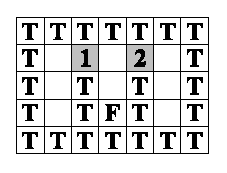
\includegraphics[width=0.26\textwidth]{woods101a.eps}}\hfill
  \subfigure[Sensory configuration of the two aliasing positions]{
  	\label{figure:woods101b}
  	
\includegraphics[width=0.15\textwidth]{woods101b.eps}}\hfill
  \caption{Trees are marked with T, food is marked with F.}
  \label{figure:woods101}
\end{figure}


Using records of past situations/actions by adding temporary memory is a
widespread approach to cope with such environments, as investigated in
\cite{Lan98,LW00}.

A second non Markov property is still embedded in \emph{multi-agent} environments and this is related to a change of an agent's internal state. In scenarios with more than one learning agent, an agent has to evaluate actions that may be caused by its own internal state or that are the result of other agent's actions. It is difficult to recognize an environmental change, which is caused by the change of another agent's internal state, due to a lack of the other agents' informations. Even if an agent stays in the same location the agent cannot evaluate the environmental changes. In \cite{TTS01}, this second non Markov property is defined as the \emph{non observable Markov decision process (NOMDP)}. 

Later in Section~\ref{subsection:scenario_classification} it will be shown that the multi-agent scenario that is presented in the next Section~\ref{section:the-predator-prey-example} includes both non Markov properties (POMDP and NOMDP). Thus learning in such an environments is more complex than learning in single-agent environments and requires a different approach which will be discussed in Section~\ref{section:reward_function}.


\section{The Predator/Prey Example}
\label{section:the-predator-prey-example}

As an example of a multi-agent approach, the predator/prey domain is an appropriate example that has successfully been studied in a variety of instantiations. It does not serve as a complex real world domain, but as a test scenario for demonstrating and evaluating manifold research ideas. Introduced by \cite{BJD86}, researchers have investigated different instantiations of its original formulation in the context of different application areas. 

Both, predator and prey, typically can move into four different directions -- north, east, south, and west. Mostly, predators follow a capturing strategy as a goal, while the prey randomly moves or stays still with a certain probability in order to simulate slower movements than the predators. A variation is that the prey moves faster than the predators. In this case a strategic collaborative effort is required by the predators. An active escaping strategy where the prey adapts and learns its behavior may also be possible.

%Worlds with other shapes as spaces (e.\,g., squares) or continuous/toroidal worlds without edges (predators and prey can move off one end of the world and come back on another end) are possible. 

%The predators try to capture the prey in such a way that the prey cannot move to an unoccupied position. If the grid world has edges, it might be possible that fewer than four predators can catch the prey by surrounding the prey against an edge of obstacles or in a corner of the world. Other parameters of the predator/prey domain are: Do the agents move simultaneously or successively -- one after the other? Is the local view of an agent limited or does an agent see the whole environment? And last, but not least, is direct communication between the agents allowed?

While predators and prey(s) have limited actions and follow well defined objectives, the predator/prey domain is simple to understand, easy to implement, and flexible enough to demonstrate a range of different scenarios, which have been emerged over the past decades. The general approach of the predator/prey example, the possibility to customize and adopt the scenario to manifold applications, or the widespread experience that is documented, not only in multi-agent literature, result in the assumption that the predator/prey example can be used as a valid testbed for OC scenarios.

Here a simpler implementation of the predator/prey scenario is examined where the predators are rewarded for just being very close to the prey and it is not necessary to surround and catch it. The overall scenario settings are described in Section~\ref{subsection:scenario} followed by a detailed description of the obstacle configurations that were tested (see Section~\ref{subsection:scenario_obstacle}). Putting all together the properties of the scenario are then compared to the properties of environments without the Markov property (see Section~\ref{subsection:scenario_classification}) and then classified according to the results of the discussion in Section~\ref{subsection:nonmarkov_environments}.


\subsection{Scenario settings}\label{subsection:scenario}

The algorithms are tested in a simple predator/prey scenario on a torus with discrete squares. The field is a quadratic, toroidal world consisting of 16x16 squares. The prey consists of a single moving goal object which the 8 agents (the predators) have not to catch but only to keep under surveillance. A cell of the two-dimensional grid-world can only be occupied by one agent. The quality of an algorithm that controls the agents is determined by the share of the time any agent has the goal object in surveillance range. It is calculated by averaging the qualities of 10 experiments consisting of 10 runs each. Each run consists of 2,000 steps after which the scenario is reset. The individual learning experiences of the agents are retained between each run but not between each experiment.

In each time step each agent can move only to one of the four neighboring fields while the goal object can move two fields. In addition there are obstacles on the field and any movement to an occupied field fails (without any further consequences). Both the goal object and the agents have 24 binary sensors that can sense their close environment but their lines of sight are blocked by obstacles or other agents. Half of the sensors can detect objects two fields away while the other half can detect objects up to five fields away (see Figure~\ref{figure:sight_directions}). The 12 sensors for each sight range are for the four directions and the three types of objects (goal object, other agents and the obstacles).


\begin{figure}[ht]
\centerline{	
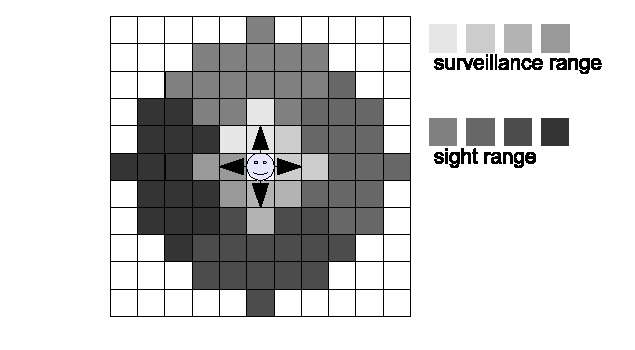
\includegraphics[width=0.4\textwidth]{sight_directions.eps}
}
\caption{Sight range ($5.0$, dark area) and surveillance range ($2.0$, bright area) of an agent / the goal object for each direction}
\label{figure:sight_directions}
\end{figure}

The simulation is conducted in discrete time. At every time step the goal object and the agents gather sensor data and decide their next actions. Then all actions of all objects are executed in a random sequence. As the goal object can move two fields it gathers new sensor data after the first step. If the goal object is surrounded by agents in all 4 directions it jumps to a random nearby free field which basically means a restart of the simulation. Experiments showed that this happened only very few times, so it does not affect the result.


\subsection{Scenario configurations}\label{subsection:scenario_obstacle}

Three different configurations of obstacles and starting positions of the agents and the goal object were thoroughly tested.

In the \emph{pillar scenario} (see Figure~\ref{figure:pillar_scenario}) there were 4 obstacles in equal distance to each other, with the goal object starting in the center and the agents starting randomly along the borders. The idea was to minimize the number of blocked fields while still giving the agents some points of orientation.

In the second scenario, the \emph{random scenario} (see Figure~\ref{figure:random_scenario}), several obstacles were placed randomly on the field, with a certain tendency to build connected structures. In both scenarios a goal object with intelligent behavior (random walk, but move away from agents in sight) and a goal object with random walk is tested. 

The third scenario, the \emph{difficult scenario} (see Figure~\ref{figure:difficult_scenario}), consisted of a cylinder and several walls with small openings. There, the goal was to find those openings that lead to the goal object which always stayed in the last section and did nothing but to move up two fields (or jump to a nearby free field if the path is blocked).

\begin{figure}[ht]
  \subfigure[Pillar scenario]{
  	\label{figure:pillar_scenario}
   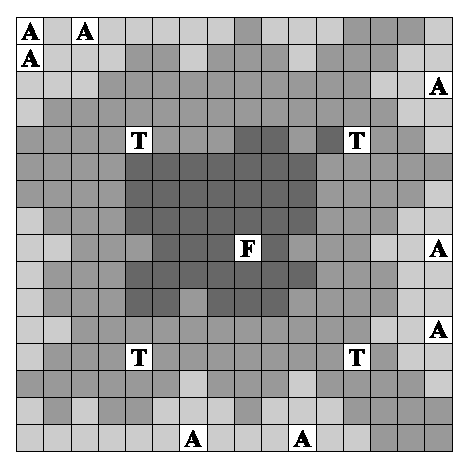
\includegraphics[width=0.14\textwidth]{pillar_scenario.eps}
  }\hfill
  \subfigure[Random scenario]{
  	\label{figure:random_scenario}
  	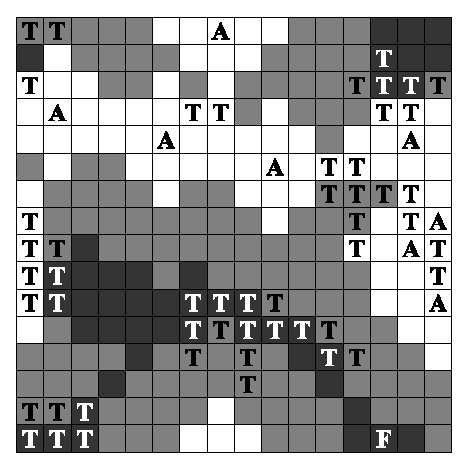
\includegraphics[width=0.14\textwidth]{random_scenario.eps}
  }\hfill
  \subfigure[Difficult scenario]{
  	\label{figure:difficult_scenario}
  	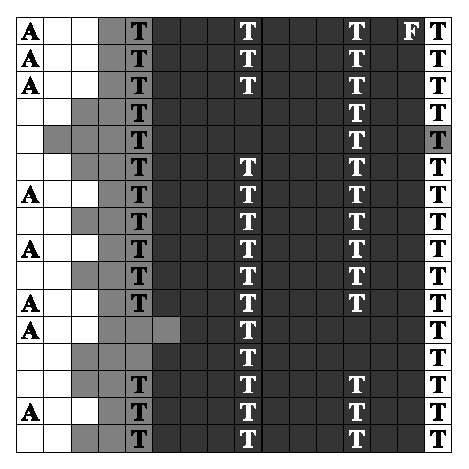
\includegraphics[width=0.14\textwidth]{difficult_scenario.eps}
  }

  \caption{These are sample start configurations for the three different types of scenarios. Trees are marked with T, food is marked with F, agents are marked with A and the surveillance and sight range is marked with light grey and grey color. Areas out of sight are marked with dark grey color.}
  \label{figure:scenarios}
\end{figure}


\subsection{Classification of the scenario}\label{subsection:scenario_classification}

As described in Section~\ref{subsection:nonmarkov_environments} environments can be classified as a MDP, a POMDP or a NOMDP. The main characteristics of a predator/prey scenario are:

\begin{enumerate*}
\item An agent has only access to local information,
\item the field usually consists of open areas with randomly placed obstacles,
\item each agent has an internal state unknown to other agents,
\item the scenario is dynamic,
\item the agents are sharing a global goal, and
\item the scenario runs continuously.
\end{enumerate*}

Clearly the scenarios in question constitute no MDPs because of limited sensory information (1, 3) and many different positions sharing the same sensory configuration (2). Because the introduction of memory would not restore the Markov property (4) it is not a POMDP either. This leaves the scenario as being a NOMDP. 

In addition special care is needed when applying XCS as is no clear local goal (5) and the scenario is not restarted when reaching the global goal (6). All in all this means that a different approach is needed and a new XCS variant needs to be created that can handle these issues properly.

In the literature NOMDP environments are discussed in connection with XCS~\cite{Miyazaki2,TTS01}. There, the issue of non observability is either evaded by a very simple scenario with only two agents or solved by using complex communication and central organization where the agents share a classifier system. Neither approach can be used here as the scenario is rather complex with many agents and there is no communication between the agents allowed. Thus it is required to develop XCS further in order to be applicable to such a dynamic collaborative scenario. The most important step is to design the reward function which will be discussed in the following section.


\section{The reward function}\label{section:reward_function}

The main prerequisite of an environment that can be solved by the single-step method is that the agent has global information. There, the optimal representation of the reward function by the XCS is also the solution of the actual problem. For example in the 6-multiplexer problem the reward function already contains the table of the 6-multiplexer itself. 

In multi-step environments the environment only returns $1$ when the agent stands on the goal position and $0$ at all other positions. As there is only access to local information it is up to the individual agent to build up a reward function for all positions in order to be able to decide which direction is to be preferred at each step.

This is done by back propagating the reward of the environment to previous actions. During the back propagation the reward is discounted in order to favor shorter routes. When the goal position is reached the scenario is repeated a number of times. In order to find the optimal (shortest) route, i.e., the global reward function, the agent must be able to distinguish between all positions, i.e., the scenario must have the Markov property.

In the predator/prey scenario the nature of the reward function is not obvious. 
In such a dynamic environment with a continuous goal condition neither repetition is possible nor does that environment possess the Markov property. Other agents and the goal object may have moved and previously gathered information might be no longer valid.

Thus, global information and therefore a global reward function cannot be constructed and it is important to reward previous actions directly. In addition it is necessary to determine points in time when a reward is to be distributed because the simulation runs continuously.

In order to fulfil these requirements a new way of reward distribution for such a scenario has been developed. First the environment reward function is chosen by testing static heuristics in the scenario (see Section~\ref{subsection:environment_reward_function}). Agents then record the resulting reward values and create \emph{events} when the values change or when there was no change for a specific amount of time (see Section~\ref{subsection:events}). After that previously executed actions are rewarded according to the type of and the time difference between the current and the last event (see Section~\ref{subsection:reward_distribution}).


\subsection{Environmental reward function}\label{subsection:environment_reward_function}

A ``goal position'' in the context of a predator/prey scenario could be defined as ``be in surveillance range of the goal object'' which would be equal to the global goal. Another approach would be to make use of the increased abilities of the sensors of the agents instead of being restricted to a simple binary function as in some multi-step environments (``goal position reached'' and ``goal position not reached''). 

Because of the number of possible reward functions that include sensory information not all functions can be tested in a reasonable amount of time. Thus, this paper proposes another approach:

By looking at the global goal it is possible to examine reward functions by testing agents with static heuristics instead of XCS. Although heuristics do not have something like a reward function as they do not learn, they still evaluate situations and corresponding actions either as ``good'' (``move in that direction'') or as ``bad'' (``don't move in that direction'').

Of a set of simple implementations the best results (except for some special cases like very large environments and a relatively small number of agents) delivered the following heuristic:

\begin{itemize}
\item Cooperation: When the goal object is not in sight move randomly in a direction without other agents in sight.
\item Egoism: Move in the direction of the goal object when it is in sight.
\end{itemize}

Modeling this heuristic would require multiple states. As the original implementation uses a binary reward function the following approximation of the reward function $r_{b}(s_{a}, s_{g})$ with $s_{a}, s_{g}$ being indicators whether the goal object is in sight range ($s_{g} = true$) and whether any other agent is in sight range ($s_{a} = true$) is used:

$$
r_{b}(s_{a}, s_{g}) = \left\{ \begin{array}{rl}
  0 & s_{a} \wedge \overline{s_{g}} \\
  1 & \overline{s_{a}} \vee s_{g}
       \end{array} \right.
$$

As further adaptions to the reward is necessary the value this function returns will be called ``base reward'' and the function itself ``environmental reward function''. In the following section the actual reward for the rules of the XCS will be calculated. 

\subsection{Events}\label{subsection:events}

Above we concluded that it is important to determine points in time when the reward is distributed. In the usual implementation of XCS~\cite{BW02} this happens whenever a positive reward is generated and the scenario is then restarted. Here, we analyze past base reward values and generate so called \emph{events} when either the \emph{base reward} value has changed or when there was no change for a certain period of time.

Assuming that the agent did something right when it gets into sight range of the goal object (or leaving the sight range of all other agents) such a situation change will be called a ``positive event'' while loosing the goal object or getting into sight range of other agents will be called a ``negative event''. Thus a positive event occurs whenever the base reward changes from $0$ to $1$, a negative event occurs whenever the base reward changes from $1$ to $0$ (see Figure~\ref{figure:positive_negative_events}).

\begin{figure}[ht]
\centerline{	
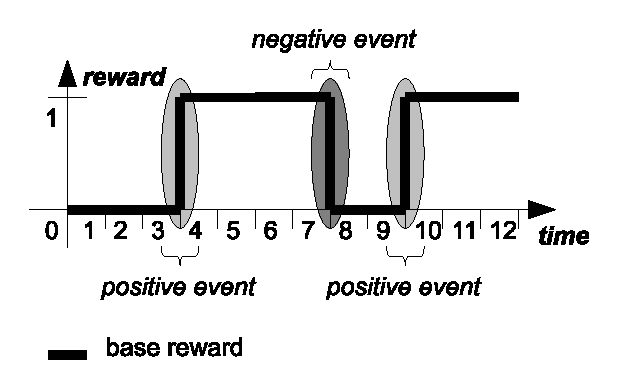
\includegraphics[scale=0.75]{positive_negative_events.eps}
}
\caption{Example of a series of base rewards that lead to positive and negative events.}
\label{figure:positive_negative_events}
\end{figure}


As there can be cases where an agent never encounters an event the number of steps is limited to \emph{maxStackSize} steps. If the step counter reaches that number then a ``neutral event'' occurs (see Figure~\ref{figure:neutral_event}). In that case the step counter is reset to $0$ and the classifier system waits for a new event or until the step counter again reaches the value of \emph{maxStackSize}. In addition half of action sets in the stack are rewarded according to the \emph{base reward} and then discarded.

\begin{figure}[ht]
\centerline{	
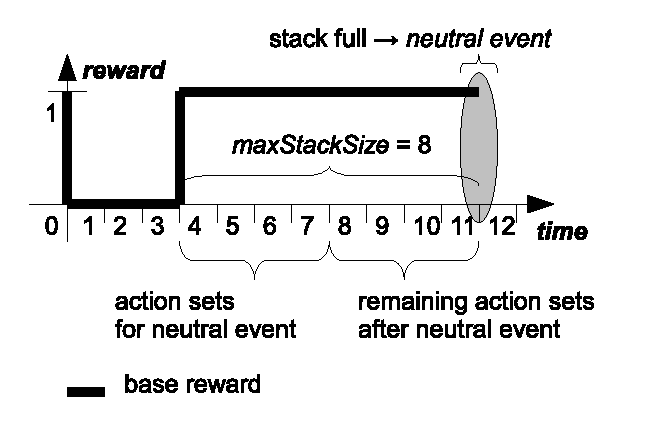
\includegraphics[scale=0.75]{neutral_event.eps}
}
\caption{Example of a series of base rewards that lead to neutral event (with \emph{maxStackSize} = 8).}
\label{figure:neutral_event}
\end{figure}


\subsection{Reward distribution}\label{subsection:reward_distribution}

The standard implementation of XCS is based on the assumption that it works in an environment with the Markov property. This is expressed in the way the reward is distributed between the classifiers that contributed to reaching the goal. It requires several repetitions in order for the reward to be transferred to all classifiers that contributed to the solution.

In the dynamic predator/prey scenario such repetitions are not available, the scenario is not restarted and runs continuously. This is the reason why separate measures have to be taken in order to reward previous contributing steps as well.

The approach that was used in this paper is to record not only the last action but all past actions. Such a memory mechanism does not necessarily restore the Markov property because the scenario is a NOMDP. But it does restore a direct connection of the reward between the goal and previous steps that contributed to the success (or failure) and an improvement in the performance is to be expected.

Thus, whenever (and only then) an event occurs, the reward is distributed among the entries of the action sets that were saved since the last event. With the idea in mind that recent actions probably contributed more to a positive (negative) event they are given a higher (lower) reward than to actions that were executed long time ago. 

This is done with a quadratic function, i.e., with \(r(a)\) being the \emph{reward} for the \emph{action set} with age \(a\):
$$
r(a) = \left\{ \begin{array}{rl}
  \frac{{a}^{2}}{{\mathrm{size(\emph{action set})}}^{2}} &\mbox{ \emph{positive event}} \\
  \frac{{(1 - a)}^{2}}{{\mathrm{size(\emph{action set})}}^{2}} &\mbox{ \emph{negative event}} \\
  1 &\mbox{ \emph{neutral event}, \emph{base reward} = $1$} \\
  0 &\mbox{ \emph{neutral event}, \emph{base reward} = $0$}
       \end{array} \right.
$$

The idea behind using a quadratic function is that it loosely resembles the transfer of the reward in the original implementation. Figure~\ref{figure:saved_rewards} shows a distribution of the reward for an exemplary distribution of the base reward. For simplicity a linear distribution is displayed in the graphics.

More sophisticated approaches are possible, this is merely the most straightforward approach. Compared to a linear distribution tests showed no significant difference. 

\begin{figure}[ht]
\centerline{	
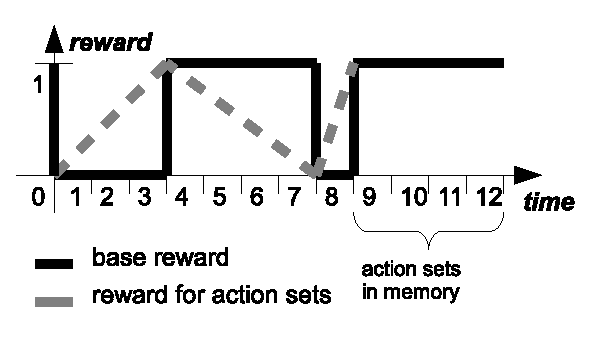
\includegraphics[scale=0.75]{saved_rewards.eps}
}
\caption{Schematic presentation of the reward distribution to the action sets over time after several positive and negative events}
\label{figure:saved_rewards}
\end{figure}



\section{Experimental results}\label{section:experiments}

Many different combinations of the reward function adaptions discussed above are possible. The main goal of this paper is to show that there are better implementations than XCS, not to find the best possible implementation. Therefore, this paper concentrates on the comparison of the XCS variants presented in the following Section~\ref{subsection:xcs_variants}.

In order to properly compare them it was important to determine good parameter settings for each variant. While most of the standard values given in~\cite{BW02} (``Commonly Used Parameter Settings'') showed good results, some special settings need closer examination. Although thousands of different combinations were tested, the parameter discussion is not necessarily complete. Of main importance was that any score below the algorithm with randomized movements has to be dismissed as it is difficult to say if a parameter settings with better results (below the result of the random algorithm) just makes the agent move more randomly or if it actually learns better. The results of the parameter discussion is described in Section~\ref{subsection:xcs_parameters}.

In the subsequent sections first the experiments with heuristics are examined (see Section~\ref{subsection:experiments_heuristics}) which is important to determine a good heuristic for the environmental reward function in Section~\ref{subsection:environment_reward_function}. Then the three scenarios discussed in Section~\ref{subsection:scenario_obstacle} are discussed: The pillar scenario (Section~\ref{subsection:xcs_pillar_scenario}), the random scenario (Section~\ref{subsection:xcs_random_scenario}) and the difficult scenario (Section~\ref{subsection:xcs_difficult_scenario}).

\subsection{XCS variants}\label{subsection:xcs_variants}

Many different combinations of the reward function options discussed in Section~\ref{section:reward_function} are possible. Surprisingly no reward function option on its own showed a better performance, using the collaborative environment reward function from Section~\ref{subsection:environment_reward_function} even reduced the performance. The best results showed a standard implementation of XCS with an environmental reward function that returns 1 when the goal object is in surveillance range and 0 at all other times.  

Using the collaborative environment reward function in connection with events (see Section~\ref{subsection:events}) and the reward distribution based on the generated events (see Section~\ref{subsection:reward_distribution}) results in the new XCS variant which will be called SXCS (\emph{Supervising eXtended Classifier System}). This variant showed significant better performance than any of the other XCS variants. The results will be presented in the following sections.


\subsection{XCS parameters}\label{subsection:xcs_parameters}

The parameter \emph{maxStackSize} that was introduced in section~\ref{subsection:events} determines when the stack overflows and a neutral event occurs. In this paper a relatively good value was determined by several experiments but further research is needed in that direction. A compromise between several conflicting factors has to be made: Large values may lead to a delay between the rewarding situation and the actual reward and the reward of uninvolved rules. On the other hand, small values may lead to early stack overflows and a possible disregard of rules that are crucial to solve the problem. As Figure~\ref{figure:max_stack_size} shows the value does not have a large impact in the pillar or random scenario, only at around \emph{maxStackSize}~\( = 8\) a difference can be seen. The difficult scenario on the other hand favors a larger value (\emph{maxStackSize}~\( = 32\)), so the optimal value depends on the scenario.

%TODO:maxStackSize 2-1024 im S�ulenszenario, Schwierigen Szenario, S�ulenszenario mit 32x32, jeweils Intelligent, Geschwindigkeit 1
%+ Random als Vergleich
%TODO bei schwierigem Szenario beachten: maxStackSize auf 32

\begin{figure}[ht]
\centerline{	
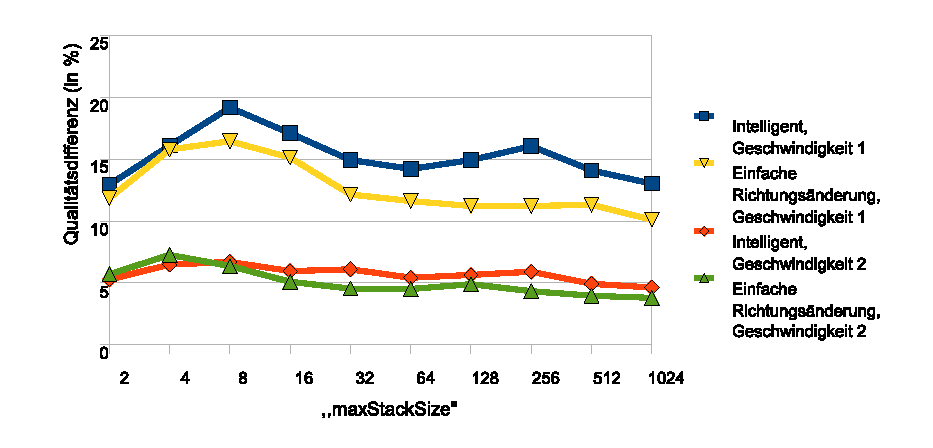
\includegraphics[scale=0.6]{max_stack_size.eps}
}
\caption{Comparison of different values of \emph{maxStackSize} in various scenarios}
\label{figure:max_stack_size}
\end{figure}


%\subsection{Learning rate $\beta$}\label{subsection:learning_rate}

During the tests another important parameter was the learning rate $\beta$. In a similar type of scenario in~\cite{1102281} a value below the standard value was proposed (\(\beta = 0.02\)). The reason was that dynamic multi-agent systems can be described only by movement probabilities so the learning process has to be slow and careful. Tests (see Figure~\ref{figure:pillar_learning_rate_quality}) showed an optimal value between \(0.01\) and \(0.1\) for SXCS, larger values seem to harm the learning process significantly. For XCS on the other hand the quality increases with larger values for \(\beta\) in this scenario. This is still a subject of research, but because larger values result in loss of comparability with other implementations of XCS the standard value of \(0.2\) was used.

%TODO beide Szenarien!

\begin{figure}[ht]
\centerline{	
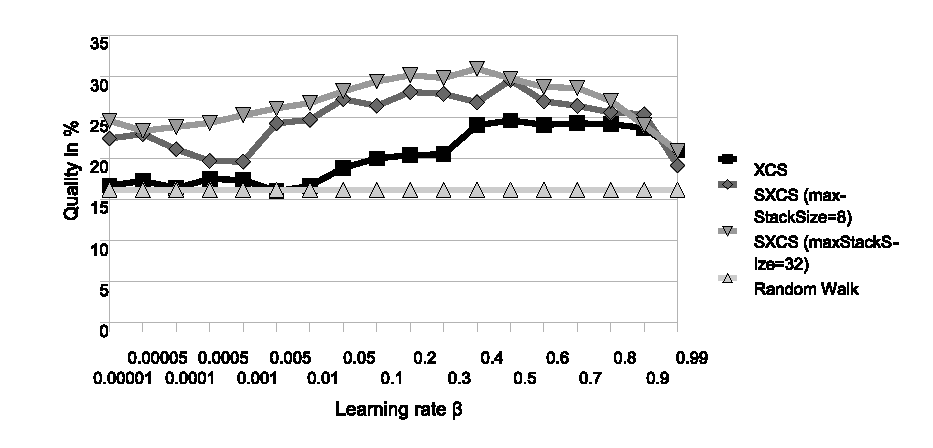
\includegraphics[scale=0.6]{learnrate_beta.eps}
}
\caption{Influence of the learning rate parameter $\beta$ on the performance (pillar scenario with XCS and SXCS agents and \emph{best selection})}
\label{figure:pillar_learning_rate_quality}
\end{figure}

According to~\cite{BW02} the maximum number of classifiers $N$ should be chosen big enough so that \emph{covering} happens only in the beginning of a run. For the scenario in question tests have shown that a population size of around $512$ fulfills this criteria. Although random initializations are possible~\cite{Butz2006}, it was chosen to start with empty classifier sets as tests have shown better performance. 

The \emph{GA threshold} parameter $\theta_{\mathrm{GA}}$ was set to $25$, larger values seemed to reduce the quality of the algorithm. As SXCS itself does use the quadratic reward distribution, the parameter \emph{reward prediction discount} $\gamma$ is only needed to compare XCS with SXCS. Tests have been inconclusive so the standard value of \(\gamma = 0.71\) was used. Only \(\gamma = 1.0\) showed significant different results, so it seems that while the reduction of the transfer of the reward is needed, the actual value is of little importance. 

Table~\ref{table:lcs_parameter} show the special settings that were used.

\begin{table}[ht]
\caption{Used parameter values and standard values}
\centering
\begin{tabular}{c c c}
\hline\hline
Parameter & Value & Standard (see~\cite{BW02})\\ [0.5ex]
\hline
max population \(N\) & \textbf{512} & [-]\\
subsumption threshold \(\theta_{\mathrm{sub}}\) & 20.0 & [20.0+]\\
GA threshold \(\theta_{\mathrm{GA}}\) & 25 & [25-50]\\
mutation probability \(\mu\) & \(0.05\) & [0.01-0.05]\\
reward prediction discount \(\gamma\) & 0.71 & [0.71]\\
learning rate \(\beta\) & \textbf{0.01 - 0.2} & [0.1-0.2]\\
tournament factor & 0.84 & [-]\\ [0.5ex]
\hline
\end{tabular}
\label{table:lcs_parameter}
\end{table}



\subsection{Experiments with heuristics}\label{subsection:experiments_heuristics}

The results displayed in Figure~\ref{figure:experiment_heuristics} show clearly that an agent with the collaborative heuristic is superior. 

\begin{figure}[ht]
\centerline{	
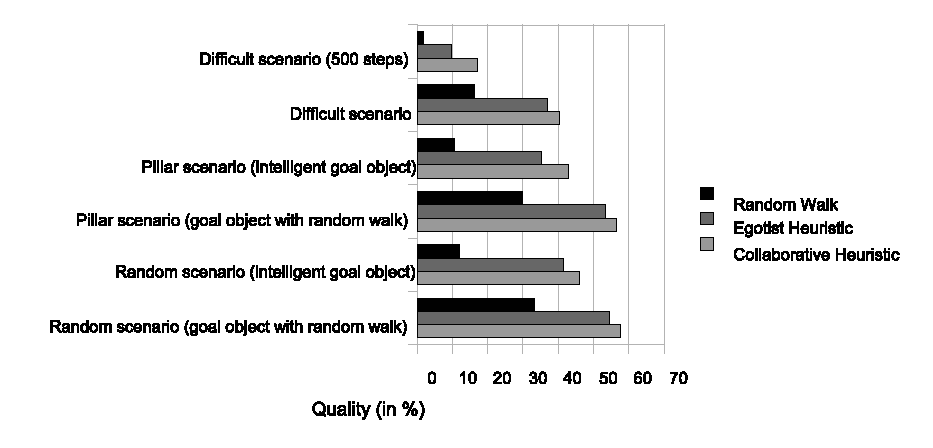
\includegraphics[scale=0.6]{experiment_heuristics.eps}
}
\caption{Comparison of different static heuristics}
\label{figure:experiment_heuristics}
\end{figure}


\subsection{Comparison in the pillar scenario}\label{subsection:xcs_pillar_scenario}
TODO

\begin{figure}[ht]
\centerline{	
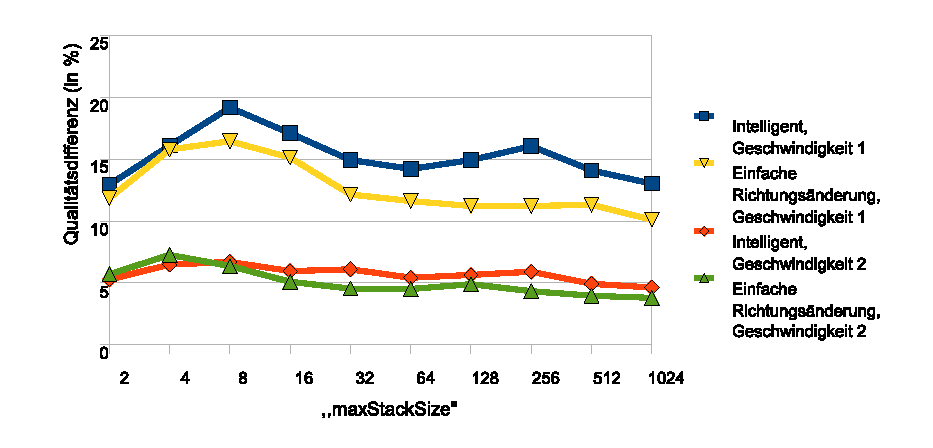
\includegraphics[scale=0.6]{experiment_pillar_scenario.eps}
}
\caption{Comparison of different XCS variants in the pillar scenario}
\label{figure:experiment_pillar_scenario}
\end{figure}

See Figure~\ref{figure:experiment_pillar_scenario}




\subsection{Comparison in the random scenario}\label{subsection:xcs_random_scenario}
TODO

\begin{figure}[ht]
\centerline{	
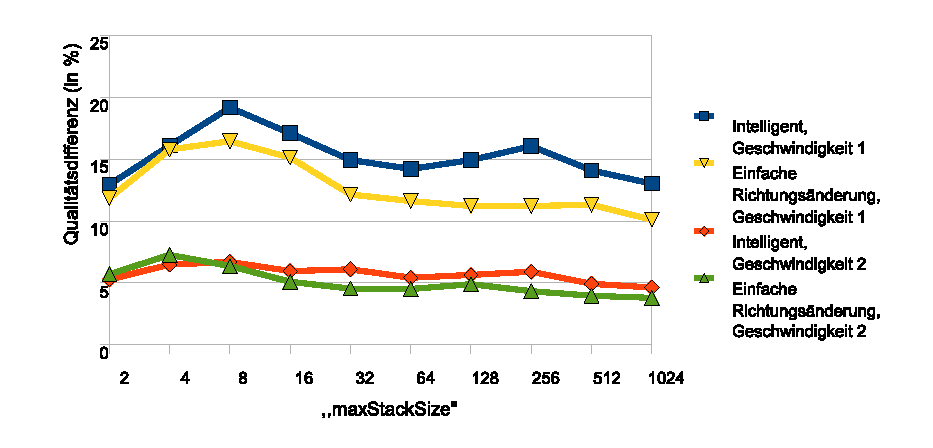
\includegraphics[scale=0.6]{experiment_random_scenario.eps}
}
\caption{Comparison of different XCS variants in the random scenario}
\label{figure:experiment_random_scenario}
\end{figure}

See Figure~\ref{figure:experiment_random_scenario}




\subsection{Comparison in the difficult scenario}\label{subsection:xcs_difficult_scenario}
TODO

\begin{figure}[ht]
\centerline{	
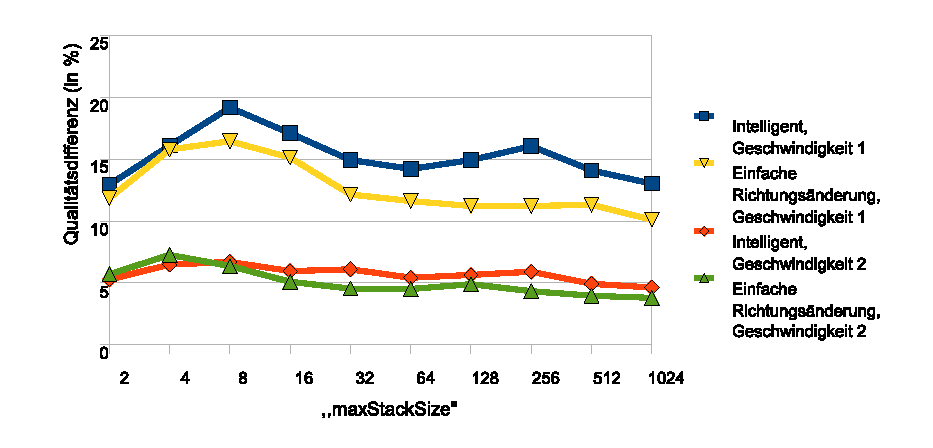
\includegraphics[scale=0.6]{experiment_difficult_scenario.eps}
}
\caption{Comparison of different XCS variants in the difficult scenario}
\label{figure:experiment_difficult_scenario}
\end{figure}

See Figure~\ref{figure:experiment_difficult_scenario}





\section{Conclusions}\label{section:conclusions}

In Section~\ref{section:experiments} it was shown that SXCS with the adapted reward function outperforms XCS.

TODO Text

All in all the results of this paper are:

TODO erst am Schlu� :)


%\begin{itemize}

%\item A good local evaluation function for the XCS can be constructed on the base of a heuristic with good performance (see Section~\ref{subsection:environment_reward_function}).

%TODO!
%\item By adding external memory that records the reward history (see Section~\ref{subsection:reward_distribution}) the newly created algorithm SXCS can solve the problem much better than XCS (see Section~\ref{section:experiments}).

%\item A variation of the learning rate $\beta$ can be successful depending on the scenario (see Section~\ref{subsection:learning_rate} and Section~\ref{subsection:xcs_difficult_scenario} for the difficult scenario respectively).

%\item Die Agenten mit XCS und SXCS haben deutliche Probleme mit Szenarien mit vielen Hindernissen (siehe Kapitel~\ref{subsection:tournament_factor_test}). TODO

%\item Ein dynamischer Wechsel der Auswahlart f�r Aktionen w�hrend eines Laufs kann sinnvoll sein, um die Zahl der blockierten Bewegungen zu verringern und das Zielobjekt besser verfolgen zu k�nnen (siehe Kapitel~\ref{subsection:analysis_random_scenario_xcs}). TODO

%\item XCS as well as SXCS can solve difficult scenarios with positions of interest significantly better than randomly moving agents. Under certain circumstances SXCS can solve this scenario even better than the heuristic on which its evaluation function is based on (see Section~\ref{subsection:xcs_difficult_scenario}).

%\end{itemize}

%binary function
%This causes some problems when trying to model the heuristic as it is impossible to distinguish situation with e.g. one other agent and four other agent in sight. Probably a better implementation would be to count the number of agents and return it as a reward. An additional problem surfaces in scenarios with a relatively low number of agents because the reward function returns 1 most of the time. This could harm the learning process.




%\begin{figure}[ht]
%\centerline{	
%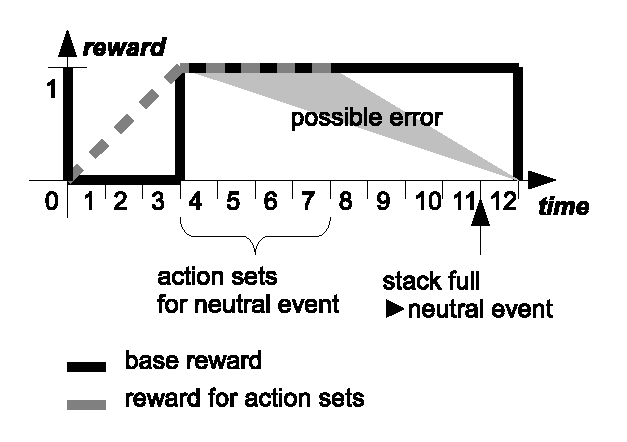
\includegraphics[scale=0.75]{neutral_reward.eps}
%}
%\caption{Schematic display of the reward distribution to the action sets after a neutral event (with \emph{base reward} = 1)}
%\label{figure:neutral_reward}
%\end{figure}


%In XCS wird lediglich die jeweils letzte \emph{action set} Liste aus dem vorherigen Schritt gespeichert. In der neuen Implementierung werden dagegen eine ganze Anzahl (bis zum Wert \emph{maxStackSize}) von \emph{action set} Listen gespeichert. Die Speicherung erlaubt zum einen eine Vorverarbeitung des \emph{reward} Werts anhand der vergangenen Schritte und auf Basis einer gr��eren Zahl von \emph{action set} Listen und zum anderen die zeitliche Relativierung einer \emph{action set} Liste zu einem Ereignis. Die \emph{classifier} werden dann jeweils r�ckwirkend anhand des jeweiligen \emph{reward} Werts aktualisiert, sobald bestimmte Bedingungen eingetreten sind.\\

%Bei der Benutzung eines solchen Stacks entsteht eine Zeitverz�gerung, d.h. die \emph{classifier} erhalten jeweils Informationen, die bis zu \emph{maxStackSize} Schritten zu alt sein k�nnen. Tritt beim Stack ein �berlauf auf, gab es also \emph{maxStackSize} Schritte lang keine �nderung des \emph{base reward} Werts mehr, dann wird abgebrochen und die \(\frac{maxStackSize}{2}\) �ltesten Eintr�ge werden vom Stack genommen. Alle diese Eintr�ge werden dabei vorher mit einem \emph{reward} Wert aktualisiert, der diesem \emph{base reward} Wert entspricht.\\

%In such a case 

%There are two drawbacks with this implementation: Firstly there is a time delay of the reward distribution because it is impossible to foresee when an event will occur. Secondly, in the case of a neutral event, the prediction of future events could be wrong and a new positive or negative event occurs shortly after the neutral event (see Figure~\ref{figure:neutral_reward}). Both points do not seem significant because the time delay, compared to the standard implementation with repetition of the problem, is very small and the erroneous reward distribution in the case of a neutral event could be corrected retroactively to a certain degree. On the other hand recording the history of rewards could provide a basis for a deeper analysis resulting in a better reward distribution than the one that is presented here.

%\subsection{Implementation of SXCS}

%The original implementation~\cite{But00} of XCS allows a modular setup of the environment so that the reward function (see Section~\ref{subsection:reward_function}) can be calculated in the environment module. As explained in Section~\ref{subsection:reward_distribution} and ~\ref{subsection:events} additional recording and analysis of the base reward generated by the reward function is necessary. Thus some parts of the code need to be rewritten resulting in the following modified version of the code:
%TODO Code?

\bibliographystyle{abbrv}
\bibliography{sigproc}


\end{document}
